\section{Funzionalità dell'editor}
\label{sec:chapter_creazione_scena_funzionalita_editor}

Allo stato attuale il servizio di editor si mostra come in figura \ref{fig:editor_1} :
\begin{figure}[h]
 \centering
 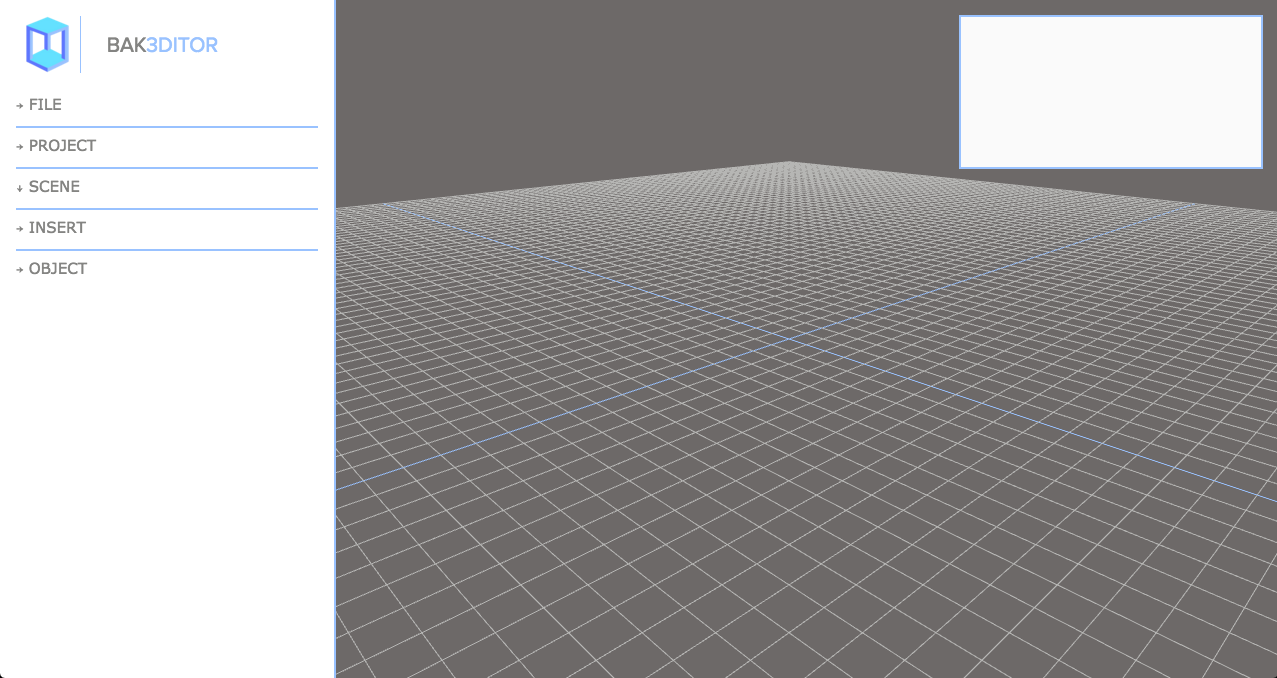
\includegraphics[width=1\linewidth]{images/chapter_creazione_scena/editor_1.png}\hfill
 \caption[Editor: stato attuale]{Impostazione attuale dell'editor}
 \label{fig:editor_1}
\end{figure}
in parte centrale è presente la vista 3D dove viene renderizzata la scena che si sta costruendo. In alto a destra una piccola mappa 2D riprende la scena dall’alto, per avere una vista planimetrica della scena. A sinistra è presente invece la barra degli strumenti, che racchiude tutte le funzionalità offerte dall’editor.
\\
Tali funzionalità si dividono in cinque categorie principali:
\begin{itemize}
\item File: Tutte le funzionalità relative all’importazione o esportazione di oggetti all’interno della scena. In particolare le opzioni \emph{save} e \emph{open catalog} saranno oggetto di analisi più approfondite in questo capitolo.
\item Project: Tutte le funzionalità che coinvolgono l’intero progetto in corso di sviluppo, come la possibilità di modificare la griglia nella canvas, o la modalità di trasformazione. Project è inoltre la categoria delle funzionalità in assoluto più importanti dell’editor, ossia quelle per la gestione del servizio di bake, e saranno anch’esse oggetto di discussioni più approfondite nel corso del presente elaborato.
\item Scene: Una lista rappresentante lo stato della scena. Ogni oggetto aggiunto alla scena è inserito nella lista; la selezione di un oggetto nella canvas comporta l’evidenziazione dello stesso nella lista; al contrario la selezione di un oggetto nella lista comporta la selezione dello stesso nella canvas. 
\item Insert: Tutte le funzionalità relative all’inserimento di oggetti all’interno della scena. Ad esempio è possibile inserire le forme geometriche o le sorgenti luminose standard di ThreeJS. Tra le geometrie è offerta anche un’opzione per l’inserimento semplificato di mura, con relativa sede per finestre o porte.
\\
Il menu insert fornisce inoltre gli strumenti per inserire una skybox all’interno della scena; questa funzionalità è del tutto nuova, e la sua implementazione, così come quella per l’inserimento dei muri, sarà descritta nei paragrafi successivi.
\item Object: Pannello delle proprietà contestuali all’oggetto attualmente in selezione. Gli oggetti selezionabili all’interno di una scena realizzata nell’editor sono Mesh o Luci; di conseguenza le proprietà nel pannello Object possono essere inerenti a:
\begin{itemize}
\item Geometria e materiale della mesh: E’ possibile applicare trasformate sulla geometria dell’oggetto (rotazione, scalatura, traslazione), così come stabilire la partecipazione o meno della mesh al processo di bake mediante i parametri \texttt{project\_shadow} o \texttt{avoid\_bake} , già menzionato nel paragrafo \ref{sec:chapter_baking_service_pipeline_baking_ciclo_bake} . Per quanto riguarda il materiale è possibile definirne il tipo tra quelli standard offerti da ThreeJS, e per ognuno modificarne le proprietà che lo caratterizzano, come il colore. Inoltre è possibile texturizzare le superfici dell’oggetto, e tra le normali opzioni di texturizzazione come l’aggiunta di una diffuse map, viene offerta anche un’opzione per generare automaticamente sull’oggetto le già menzionate envmap di riflessione o rifrazione. I dettagli implementativi di quest’ultma opzione verranno discussi nel paragrafo \ref{sec:chapter_creazione_scena_funzionalita_editor_envmap} .
\item Sorgente luminosa: E’ possibile configurare tutte le proprietà standard delle luci in ThreeJS, come colore e intensità. Anche qui vi sarà un paragrafo dedicato, il \ref{sec:chapter_creazione_scena_mapping_illuminazione} , per l’adattamento delle luci in ThreeJS al sistema di illuminazione di Blender.
\end{itemize}
\end{itemize}
E’ importante ricordare il fatto che ogni funzionalità menzionata fin’ora è rappresentata da un web component. Ognuna di queste è dunque un modulo implementato come entità a se stante, che racchiude solamente le responsabilità funzionali di implementare l’azione per cui è stato ideato, senza dipendere dalle responsabilità di altri elementi.
\\
I prossimi paragrafi prenderanno in esame ognuna delle componenti fondamentali di cui si è fatto menzione nel presente paragrafo.

\subsection{Salvataggio di una scena}
\label{sec:chapter_creazione_scena_funzionalita_editor_salvataggio_scena}
In ogni fase della costruzione di una scena 3D da parte dell’utente deve essere possibile salvare il lavoro svolto, memorizzando non solo gli oggetti che fino a quel momento sono stati aggiunti alla scena, ma anche tutte le proprietà che li caratterizzano, come trasformazioni sulle relative geometrie, proprietà dei materiali, o informazioni sulle sorgenti luminose. 
\\
La funzionalità di salvataggio della scena si basa su un esportatore preesistente fornito da ThreeJS, al quale però sono state aggiunte due funzionalità per un preprocessamento di alcuni attributi della scena prima della vera e propria esportazione.
\\
Compito di questo paragrafo sarà descrivere e motivare le funzionalità aggiunte, iniziando dal preprocessamento delle geometrie degli oggetti che popolano la scena.
\\
Come già discusso nel paragrafo \ref{sec:chapter_architettura_sistema_formato_scambio} , per far si che la scena salvata sia interpretabile dal servizio di baking, così come dal navigator, si è scelto un formato di scambio dei dati univoco.
\\ 
Questo formato di scambio prevede che le geometrie vengano rappresentate da una classe alternativa alla \texttt{Geometry} standard di ThreeJS, detta \texttt{THREE.BufferGeometry}.
La caratteristica chiave di una BufferGeometry è che i dati, come la posizione dei vertici, gli indici di faccia, le normali, il colore, e le coordinate UV, vengono memorizzati all’interno di buffer. 
\\
Questo formato di memorizzazione riduce il costo di trasferire le informazioni geometriche all’hardware di accelerazione grafica, in quanto WebGL utilizza il medesimo formato di rappresentazione dei dati. La classe BufferGeometry è stata infatti realizzata conseguentemente alla nascita di WebGL, e fa si che il renderer, prima di trasferire i dati geometrici allo shader, non li deve bufferizzare, cosa che avrebbe dovuto fare utilizzando la classe Geometry.
\\
Tale caratteristica rende tuttavia la BufferGeometry una classe molto più complessa da utilizzare rispetto ad una Geometry.
\\
Ad esempio la posizione di un oggetto nello spazio 3D della scena non è accessibile
mediante apposito vettore posizione a tre componenti, ma dovrà essere estratta da un buffer grezzo contenente tutte le informazioni di trasformazione, richiedendo inevitabilmente un maggiore sforzo produttivo.
\\
Per questo motivo è preferibile utilizzare la classe BufferGeometry quando si ha a che fare con oggetti statici, le cui geometrie non devono quindi essere manipolate dopo l’istanziazione dei relativi oggetti.
\\
Nel contesto del presente elaborato di tesi è stato adottato un’approccio per cui, nel momento in cui viene esportata la scena, ogni geometria viene convertita in BufferGeometry.    
\\
La procedura di esportazione della scena prevede che l’intero albero degli oggetti che la compongono venga dapprima convertito in un oggetto descritto in formato JSON; tale oggetto viene poi tradotto in stringa e scritto in un file con estensione .json. La procedura di conversione in BufferGeometry è collocata prima della traduzione dell’albero della scena, e consiste nell’individuare all’interno di essa tutte le Mesh, e per ognuna di queste estrarre la relativa geometria e darla in input al metodo \texttt{fromGeometry()} della classe \texttt{THREE.BufferGeometry()}. 
\\
\\
Oltre alla conversione in BufferGeometry, il processo di esportazione prevede un preprocessamento anche del base64 delle immagini con cui sono texturizzate le superfici degli oggetti all’interno della scena. 
\\
Se si accede alla proprietà \texttt{image} di una diffuse texture applicata al materiale di un oggetto, è possibile trovarvi un elemento HTML con tag \texttt{<image>} ed attributo \texttt{src} uguale al data URL dell’immagine. Questo data URL si è scoperto avere una dimensione minore di quello che veniva memorizzato nel JSON nel momento in cui, durante il processo di esportazione della scena, il relativo albero degli oggetti veniva tradotto nel suddetto formato. Questa situazione, se si considera la texturizzazione di un elevato numero di oggetti all’interno della scena, comporta inevitabilmente l’esportazione in .json sovradimensionati. 
\\
Pertanto, a seguito della conversione in JSON dell’albero della scena, e prima della relativa traduzione in stringa, ogni data URL sovradimensionato contenuto nell’attributo image del JSON viene sostituito con il più piccolo data URL contenuto nell’attributo src dell’elemento HTML <image> rappresentate la stessa immagine.
\\
Tale procedura permette quindi di ottenere un file .json dalle dimensioni ridotte, il che ne semplifica inoltre il trasferimento al servizio remoto di baking. 

\subsection{Componibilità e Catalogo prodotti}
\label{sec:chapter_creazione_scena_funzionalita_editor_catalogo}
Nell’introduzione si è fatta menzione alla possibilità dell’editor di poter essere esteso nelle funzionalità che offre, mediante l’integrazione di widget.
\\
Durante la realizzazione del sistema trattato nel presente elaborato di tesi, l’editor ha potuto ricevere sin da subito dei contributi volti a estenderne le funzionalità per quanto riguarda l’arredamento di interni 3D.
\\
Obiettivo finale è infatti quello di ottenere un editor ricco di funzionalità volte a migliorare l’esperienza utente dedito alla realizzazione e all’arredamento di interni 3D, come la possibilità di fruire di setup di arredamento preimpostati in base all’ambiente della casa, aiutare l’utente nell’abbinamento e nel posizionamento degli oggetti, fornire un catalogo di prodotti d’arredo pronti all’uso, o un sistema per semplificare la realizzazione delle mura domestiche.
\\
Ognuna di queste funzionalità può essere implementata separatamente, ed inclusa in un elemento html custom da importare all’interno dell’editor.
\\ 
Inoltre alla realizzazione di ogni widget possono prendere parte team di sviluppo differenti, in quanto operanti su moduli completamente disaccoppiati gli uni dagli altri.
\\
\\
Nel presente paragrafo verrà descritta la prima funzionalità realizzata tra quelle sopra citate, ovvero l’inserimento nell’editor di un catalogo di prodotti per l’arredo. 
\\
Alla selezione dell’opzione \texttt{open catalog}, un elemento html rappresentante il catalogo viene mostrato su schermo. Il catalogo mostra all’utente una serie di immagini raffiguranti i modelli che il catalogo ha da offrire. L’utente può quindi scorrere tra i modelli offerti, e una volta trovato il modello di interesse può selezionarlo ed inserirlo all’interno della scena.
\\
La realizzazione del catalogo è indipendente dai modelli che contiene; questo significa che in qualsiasi momento è possibile accordarsi con un fornitore per dei modelli d’arredo, ed inserirli all’interno del catalogo.
\\ 
Il modo in cui il fornitore può mettere a disposizione i propri modelli da inserire nel catalogo è, per ogni oggetto, un file in formato .obj, una texture, e un’immagine del modello, insieme eventualmente ad una descrizione dello stesso in formato JSON.
\\
Per quanto riguarda i dettagli realizzativi, il catalogo si articola nel modo seguente.
\\
Si supponga di avere a disposizione un catalogo di prodotti, memorizzato su di una risorsa remota accessibile mediante relativa URL. Ovviamente la natura web del servizio permette di poter fruire del catalogo da remoto, e scaricare sul client solamente i modelli scelti dall'utente. Per mostrare quindi all’utente tutti i modelli del catalogo, senza doverli scaricare preventivamente, vengono mostrate lato client solo le immagini dei modelli.
Per scaricare un modello è necessario sottomettere una richiesta alla risorsa dove è memorizzato il catalogo, insieme ad un identificativo del modello stesso che si vuole scaricare. Tale identificativo, insieme all’immagine del modello, dovranno quindi essere scaricati sul client nel momento in cui l’utente accede al catalogo.
\\
L’operazione di sottomissione della richiesta viene resa completamente trasparente all’utente, che si limiterà a cliccare sulle immagini relative ai modelli che vuole inserire nella scena.
\\ 
Nel momento in l’utente seleziona il modello dal catalogo, l’editor si occupera di invocare il metodo \texttt{download\_obj}, passando come input l’identificativo del modello associato all’immagine selezionata. Tale metodo si occuperà quindi di sottomettere la richiesta al catalogo, e una volta scaricato il modello con la relativa texture provvederà ad aggiungerlo alla scena. 
\\
\\
Per la sottomissione di una richiesta a risorsa remota si è scelto di utilizzare le API \emph{Fetch} \cite{fetchapi} . Queste API espongono un’interfaccia per il fetch delle richieste attraverso la rete.
\\ 
La sottomissione di una richiesta avviene mediante il metodo \texttt{fetch()} , il quale prende come argomento il path alla risorsa dalla quale si vuole scaricare il modello. Il path consiste nell’URL alla risorsa del catalogo, concatenata all’id del modello che si intende scaricare.
\\
Una volta sottomessa la richiesta, non è possibile determinare con certezza il momento in cui tale richiesta verrà soddisfatta, e quindi non è possibile stabilire quando il modello potrà essere aggiunto alla scena.
\\
Per questo motivo il metodo fetch restituisce una promessa che la richiesta verrà elaborata in un certo modo quando, e se, questa sarà soddisfatta.
\\ 
Per associare un’azione da perseguire nel momento in cui la richiesta sarà soddisfatta, si invoca sulla promessa un metodo \texttt{then()}, che come input prende un’oggetto di tipo \texttt{Response}, e una funzione che implementa i passi di elaborazione con cui processare l’oggetto Response una volta ottenuto.
\\
Un oggetto di tipo Response offre un insieme di metodi che permettono di dichiarare il tipo di formato in cui si vogliono convertire i dati grezzi della risposta, e come questi dabbano essere gestiti.
\\
Ad esempio se si volessero convertire i dati grezzi di un’oggetto Response in un formato .obj, il metodo che verrebbe invocato sull’oggetto Response sarebbe \texttt{text()} . 
\\
Anche in questo caso verrebbe restituita una promessa, in particolare una promessa che il dato grezzo sarà convertito in testo; di conseguenza su questa promessa può essere invocato un’ulteriore metodo then(), al quale però non verrà passato un’oggetto risposta, ma l’output del passo precedente, e quindi nell’esempio un oggetto in formato testo.
\\ 
In questo modo è possibile avvalersi delle Fetch API per definire una catena di elaborazione basata su promesse.
\\  
L’utilizzo delle promesse è una scelta possibile per la realizzazione del catalogo, in quanto per scaricare obj e texture del modello sarà necessario sottomettere due richieste.
\\
Siccome un’oggetto per essere texturizzato deve trovarsi all’interno della scena, la procedura di texturizzazione potrà essere fatta solo nel momento in cui si è certi che il file obj del modello sia stato completamente scaricato e importato nella scena. In questo caso si utilizzerà dunque una promessa, che l’oggetto è stato scaricato correttamente e aggiunto alla scena. Solo in questo caso verrà eseguito il secondo fetch alla risorsa contenente la texture del modello.
La procedura di scaricamento di un modello dal catalogo è riassunta in figura \ref{fig:editor_2} .
\\
\begin{figure}[h]
 \centering
 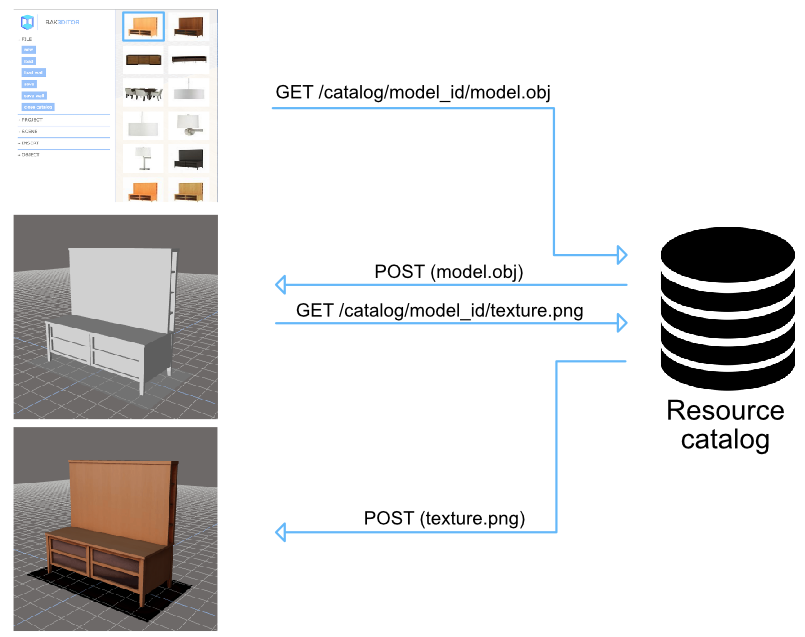
\includegraphics[width=0.7\linewidth]{images/chapter_creazione_scena/editor_2.png}\hfill
 \caption[Catalogo prodotti]{Funzionamento generale del catalogo prodotti all'interno dell'editor. Si noti come la seconda richiesta per la texture del modello venga sottomessa solamente a seguito dell'importazione nella scena dell'obj dello stesso.}
 \label{fig:editor_2}
\end{figure}

\subsection{Invocazione e gestione del processo di bake}
\label{sec:chapter_creazione_scena_funzionalita_editor_bake}
Il processo di baking delle lightmap abilita la possibilità di rendere fotorealistiche le scene 3D realizzate all’interno dell’Editor. Nel capitolo precedente si è discusso circa il modo in cui il servizio di baking ascolti le richieste dell’utente, ne riconosca la tipologia, ed invochi i relativi processi di elaborazione.
\\ 
Il tipo delle richieste al servizio di bake che l’utente sottomettere dipende dall’opzione selezionata dallo stesso all’interno dell’editor.
\\ 
Nel capitolo \ref{sec:chapter_caso_uso_creazione_scena} si è già discusso circa le opzioni dell’Editor per la gestione del processo di baking all’interno del pannello \texttt{PROJECT/bake} .
\\
La selezione dell’opzione bake, così come jobs, status, o delete, corrisponderà ognuna alla sottomissione di una richiesta di diverso tipo al servizio di baking, in modo completamente trasparente all’utente. Il meccanismo di funzionamento richiama infatti quello del catalogo mostrato nel paragrafo precedente: l’utente non vede la sottomissione di una richiesta http a servizio remoto, ma solamente il risultato su schermo scaturito da un click su una funzionalità dell'editor.
\\
Il metodo per richiedere dei servizi al server remoto sarà dunque lo stesso, ovvero il fetch di una richiesta ad un servizio.
\\ 
Alla selezione di ognuna delle opzioni all’interno del pannetto PROJECT/bake corrisponde l’invocazione di una funzione che si prenderà carico del fetch di una richiesta del tipo inerente all’opzione selezionata. Come per l’implementazione del servizio di importazione dei modelli dal catalogo, anche in questo caso si farà uso delle API Fetch, e quindi delle promesse per dichiarare dei passi di elaborazione che verranno svolti quando, e se, la richiesta sarà soddisfatta.
\\ 
A questo punto il paragrafo prenderà in esame punto per punto tutte le opzioni fornite nel pannello PROJECT/bake, descrivendo per ognuna i dettagli di funzionamento.
\\
Partendo dalla più importante, ovvero bake, la selezione della relativa opzione comporterà per prima cosa l’estrazione delle informazioni riguardanti nome della scena, sampling, ed email, immessi dall’utente nell’apposita form da compilare prima di poter invocare il comando. Una volta estratte tali informazioni, verrà invocato il metodo \texttt{bake()} , che si prenderà carico del fetch della richiesta al servizio di bake, e all’elaborazione della relativa risposta.
\\
Per sottomettere una richiesta al suddetto servizio è necessario conoscere l’indirizzo e la porta sulla quale il server è in ascolto; inoltre è necessario che il tipo di richiesta sia conforme a quella riconosciuta dallo stesso server come richiesta di bake. In particolare, facendo riferimento alla tabella \ref{table:middleware_table} di pagina \pageref{table:middleware_table} , il metodo http di una richiesta di bake è \texttt{POST} , e la rotta di destinazione è \texttt{/bake} . Ovviamente si tratta di una POST in quanto sarà necessario trasferire al servizio di bake la scena 3D sulla quale si è scelto di processare il baking delle lightmap.
\\
Le API Fetch verranno quindi utilizzate per realizzare una POST. Differentemente da quanto visto nel paragrafo precedente, dove per realizzare una GET è sufficiente invocare il metodo fetch() passando come argomento l’url della risorsa, in questo caso allo stesso metodo bisognerà passare un secondo parametro, contenente:
\begin{itemize}
\item Metodo della richiesta, quindi POST.
\item Un header dove verrà specificato il tipo di contenuto del body, quindi un file json.
\item Il body, in cui verrà inserita la scena descritta nel formato di interscambio dei dati discusso nel paragrafo \ref{sec:chapter_architettura_sistema_formato_scambio} .
\end{itemize}
L’invocazione del metodo fetch() restituirà una promessa che la richiestà verrà soddisfatta.
\\ 
Il servizio di bake si impegnerà a fornire una risposta con le informazioni relative alla richiesta elaborata, alcune delle quali sono state discusse nel paragrafo \ref{sec:chapter_baking_service_architettura_servizio} .
\\
E’ importante sottolineare che questa risposta non conterrà la scena con le lightmap, ma solo alcune informazioni relative all’accettazione della richiesta; il processo di bake potrebbe infatti avere inizio successivamente alla ricezione della risposta, a seconda del numero di processi attualmente in coda (per i dettagli si rimanda al paragrafo \ref{sec:chapter_baking_service_architettura_servizio} ).
\\ 
Sulla promessa verrà quindi invocato un metodo then(), dove verranno specificati i passi di elaborazione per quando la risposta sarà giunta al client. In particolare siccome le informazioni contenute nella risposta dovranno essere interpretate in formato JSON, il metodo then() conterrà le istruzioni per convertire i dati grezzi della risposta nel suddetto formato. Una volta ottenuto il file JSON con i dati della risposta, è possibile farne uso per notificare all’utente l’identificativo del processo di bake da lui richiesto.
\\
\\
La seconda opzione selezionabile dall’utente all’interno del pannello PROJECT/bake è quella relativa alla richiesta dei processi di bake attualmente in accettazione o in esecuzione.
In questo caso il fetch sarà per una \texttt{GET} al servizio di bake, e l’URL della richiesta sarà il medesimo, a meno della parte finale che conterrà \texttt{/jobs} al posto di \texttt{/bake}.
\\
L’output sarà nuovamente una promessa, ed anche in questo caso i dati della futura risposta saranno convertiti in JSON, in quanto rappresentanti i \texttt{bake\_data} dei processi di bake attualmente in stato di attesa o esecuzione (per maggiori dettagli sui bake\_data, si rimanda al capitolo \ref{sec:chapter_baking_service_architettura_servizio} ).
Una volta ottenuti i bake\_data l’ultimo passo di elaborazione consiste nell’estrarre da ognuno il nome della scena e memorizzarlo in una lista mostrata su schermo.
\\
\\
Per ogni job della lista vengono fornite due operazioni possibili: \emph{delete} e \emph{status}. 
\\
La selezione della prima opzione comporterà l’invocazione del metodo \texttt{delete()} che come unico argomento prende l’id del processo di bake collegato al nome della scena in corrispondenza del quale si è selezionata l’opzione delete. Tale metodo eseguirà il fetch di una richiesta di tipo \texttt{DELETE} , con URL invariato a meno della parte finale, che conterrà \texttt{/delete} concatenato all’id del processo di bake di cui si vuole richiedere l’operazione.
\\
Per la creazione di una richiesta con metodo delete bisognerà passare al metodo fetch() un secondo argomento, che a differenza di quello della POST sarà un oggetto contenente un unico campo \texttt{method} , dove appunto verrà specificato \texttt{delete} .
\\ 
Una volta mantenuta la promessa che la richiesta verrà soddisfatta, la rispostà verrà elaborata estraendo il messaggio di risposta del servizio di bake, e mostrandolo su schermo.
\\
Infine per quanto riguarda l’opzione \emph{status} la procedura è molto simile, a differenza del fatto che questa volta il metodo della richiesta è GET, e che la parte finale dell’url conterrà \texttt{/status} seguito dall’id del processo di bake. Anche in questo caso verrà estratto dalla richiesta il messaggio restituito dal servizio di bake, e mostrato su schermo. Per i tipi di messaggi che possono essere restituiti si rimanda al capitolo \ref{sec:chapter_baking_service_architettura_servizio} .

\subsection{Creazione Muri}
\label{sec:chapter_creazione_scena_funzionalita_editor_muri}
Nel presente paragrafo verrà descritta la funzionalità offerta dall’Editor per semplificare la creazione di muri all’interno della scena.
\\
Questa attività in ThreeJS può presentare delle difficoltà nel momento in cui si decide di inserire un foro per una finestra o una porta.
\\
Tale procedura può essere svolta utilizzando la classe \texttt{THREE.ShapeGeometry} offerta da ThreeJS.
\\
Un’oggetto della classe ShapeGeometry può essere posizionato all'interno della scena 3D e mosso lungo un percorso chiuso definito da un insieme di punti forniti dall’utente. Ogni coppia di punti lungo il percorso delimiterà un tratto dello stesso, che può essere visto come uno spigolo della ShapeGeometry. Alla geometria risultante possono essere aggiunti degli oggetti di tipo \texttt{Hole} , i quali vengono costruiti come le SphapeGeometry. Una volta definito all’interno di un oggetto Hole l’insieme di punti che compone il percorso delimitante il foro, tale oggetto viene aggiunto alla ShapeGeometry, ottenendo quindi una geometria bucata.
\\
La procedura appena mostrata porta alla realizzazione di una geometria bucata in due dimensioni; per ottenerne una in tre è possibile istanziare un oggetto della classe \texttt{THREE.ExtrudeGeometry}, passando come argomento l’oggetto ShapeGeometry e un’insieme di parametri per configurare il tipo di estrusione, come lo spessore che dovrà avere la geometria estrusa. 
\\
Come è possibile notare il processo può risultare difficoltoso, e per questo si è deciso di automatizzarlo.
\\ 
In particolare l’editor offre all’utente la possibilità di fruire del processo automatizzato per la creazione dei muri in due modi: il primo è selezionando l’opzione \emph{load wall} nel menu \emph{FILE} , e caricando un file JSON contente la descrizione delle mura che si vogliono costruire all’interno della scena. 
Il JSON descrive un array di oggetti wall, ognuno dei quali è composto da:
\begin{itemize}
\item Un’array di punti per disegnare la ShapeGeometry del muro.
\item Un’array di oggetti hole, ognuno dei quali è descritto da:
\begin{itemize}
\item Un’array di punti per disegnare l’oggetto Hole da aggiungere alla ShapeGeometry.
\end{itemize}
\item Lo spessore che dovrà avere il muro.
\end{itemize}
Una procedura si prenderà poi carico di leggere l’intero file JSON, e passare le informazioni alla funzione generatrice della Mesh muro, che verrà poi importata all’interno della scena.
\\
La seconda modalità è più interattiva e, come mostrato nel capitolo \ref{sec:chapter_caso_uso_creazione_scena} , prevede da subito l’inserimento di un oggetto \texttt{WALL} all’interno della scena. Trattandosi di una comune geometria standard ThreeJS può essere modellata per definire le dimensione del muro. Inoltre l’oggetto WALL è costituito da un secondo elemento \texttt{HOLE} più piccolo, il quale può a sua volta essere modellato per definire le dimensione che il foro dovrà avere. Una volta modellati HOLE e WALL, l’opzione \emph{create} provvederà a rimuoverli dalla scena, e generare la corrispondente Mesh muro. WALL e HOLE rappresentano quindi solamente degli oggetti di supporto alla modellazione della Mesh muro che verrà poi inserita all’interno della scena.
\\
Tale soluzione gode sicuramente di un’usabilità maggiore, in quanto non richiede la scrittura di un file JSON; tuttavia allo stato attuale è uno strumento meno potente, per via del fatto che per ogni muro può essere generato un solo foro. 
\\
\\
E’ importante sottolineare che, nonostante le due modalità sopra mostrate siano differenti, il processo di creazione della Mesh muro rimane identico. Ciò che cambia infatti è solamente il modo in cui l’input, ovvero le coordinate dei punti per disegnare muri e fori, e lo spessore degli stessi, viene passato alla procedura. Infatti, mentre nella prima procedura l’input viene letto da un file JSON, nel secondo caso l’input viene estratto dai dati geometrici degli oggetti WALL e HOLE.
\\ 
Per quanto riguarda la procedura automatizzata per la creazione del muro, una volta ottenuto l’input da uno dei due metodi sopra mostrati, mediante processo di iterazione sui punti che descrivono la forma in 2D del muro e dei relativi fori, verrà creato un’oggetto ShapeGeometry con cui generare, insieme allo spessore del muro, l’ExtrudeGeometry definitiva.
\\ 
Tale ExtrudeGeometry necessita di un’ulteriore passo di elaborazione:
Se si considerano delle mura domestiche, è tipicamente possibile che le due pareti che compongono alcuni muri siano diverse; questo si traduce nella necessità di dover texturizzare le due pareti del muro in maniera differente.
\\
Utilizzando una sola ExtrudeGeometry questa attività risulta impossibile, in relazione soprattutto al fatto che nel processo di baking verrebbe fatto l’unwrap dell’intera geometria, rendendo impossibile un calcolo delle lightmap diversificato su due pareti.
Pertanto si è scelto di combinare l’oggetto ExtrudeGeometry con due oggetti 2D ShapeGeometry identici al muro, entrambi posizionati in corrispondenza delle due parenti, uno con le normali di faccia in posizione frontale (\texttt{FrontSide}), l’altro con le normali invertite (\texttt{BackSide}). Quest’ultimo caso ha reso necessario l’inserimento del metodo per il flip delle normali, discusso nel paragrafo \ref{sec:chapter_baking_service_pipeline_baking_caricam_scena} . In questo modo è possibile texturizzare le pareti del muro in maniera differente, come mostrato in figura \ref{fig:editor_3} .
\\
\begin{figure}[h]
 \centering
 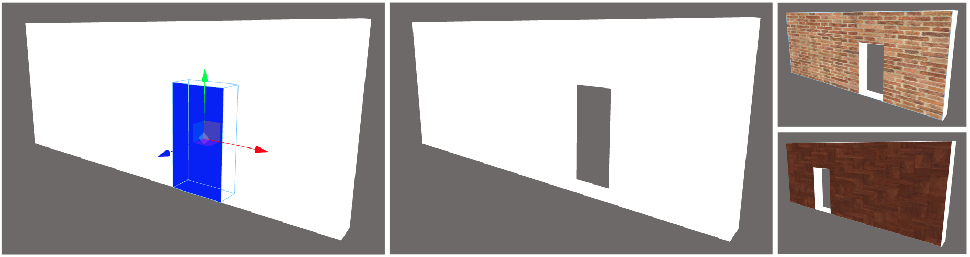
\includegraphics[width=1\linewidth]{images/chapter_creazione_scena/editor_3.png}\hfill
 \caption[Creazione muri]{Processo di creazione di un muro all'interno dell'editor, mediante funzionalità interattiva. Si noti come, nella parte destra della figura, entrambe le pareti del muro siano texturizzabili in maniera differente.}
 \label{fig:editor_3}
\end{figure}
\newpage
\subsection{Creazione Skybox}
\label{sec:chapter_creazione_scena_funzionalita_editor_skybox}
La creazione di una skybox è un metodo di ampio utilizzo specialmente in ambiente videoludico, dove il livello di gioco viene racchiuso in una forma geometrica, come un cubo, molto grande sulle cui facce viene proiettato paesaggio mediante l’utilizzo del metodo di mappatura cubica (di cui si è gia discusso nel capitolo \ref{sec:chapter_stato_arte_envmap_cubica} ). Questa tecnica conferisce l’illusione di avere a disposizione un’ambiente di gioco molto più grande di quello che effettivamente si possiede.
\\
\\
L’ambiente Editor fornisce uno strumento per la generazione delle skybox, il quale sostanzialmente consiste nello scegliere 6 texture da mappare su ogni faccia del cubo, indicando anche la posizione dove si vuole proiettare la relativa texture, e nello stabilire la dimensione della skybox. 
\\
Una volta che tali parametri sono stati configurati, l’editor si impegna nell’aggiungere alla scena e orientare 6 forme geometriche planari, che costiuiranno le facce della skybox, e nella texturizzazione di ognuna delle facce.
\\
Siccome la skybox risulta un elemento della scena, in caso di sottomissione di una richiesta di bake verrebbe passata al relativo servizio insieme ad essa. Tuttavia gli elementi della skybox non dovrebbero partecipare al processo di baking delle lightmap, pertanto è stato necessario istruire il processo di baking affinchè non considerasse gli elementi della skybox, considerandoli tuttavia per il processo di esportazione della scena finale.
\\
Per risolvere questo problema ad ogni faccia della skybox viene associato il parametro \texttt{avoid\_bake} (di cui si è già discusso nel capitolo \ref{sec:chapter_baking_service_pipeline_baking_ciclo_bake} ), tramite cui Blender è in grado di comprendere se l’oggetto deve o meno partecipare al baking delle lightmap. Siccome il parametro avoid\_bake, per essere letto da Blender, dovrà trovarsi all’interno del JSON contenente la descrizione della scena 3D, si è reso necessario modificare ThreeJS affinchè il metodo per la conversione della scena 3D in formato JSON trascrivesse anche questo nuovo parametro insieme a quelli standard per la descrizione degli oggetti. 
\\
\begin{figure}[h]
 \centering
 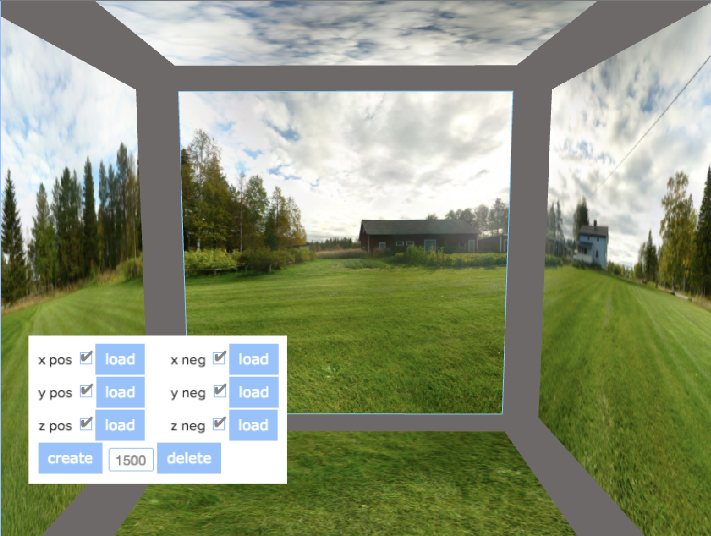
\includegraphics[width=0.8\linewidth]{images/chapter_creazione_scena/editor_4.png}\hfill
 \caption[Creazione Skybox]{Dettaglio sul pannello dell'editor dedicato alla creazione delle sei facce della skybox, e risultato corrispondente; ogni faccia è distanziata per migliorare la percezione in foto dei singoli elementi che compongono la skybox.}
 \label{fig:editor_4}
\end{figure} 

\subsection{Generazione delle env map}
\label{sec:chapter_creazione_scena_funzionalita_editor_envmap}

All’interno dell’editor è possibile creare degli effetti di riflessione o rifrazione sulle superfici della Mesh generando un’envmap di rifrazione o riflessione.
\\
I benefici nell’utilizzo di una struttura dati di questo tipo sono descritti nel capitolo \ref{sec:chapter_stato_arte_envmap}; questo paragrafo si concenterà piuttosto sul funzionamento della procedura di generazione. 
\\
Unica precondizione per generare un’envmap all’interno dell’editor, è che la Mesh sulla cui superficie si vuole mappare l’envmap sia selezionata. A seconda che l’utente voglia generare un effetto di riflessione o rifrazione, selezionerà l’apposita funzione \emph{refr} o \emph{refl} nel menu \emph{OBJECT/material}; l’editor si impegnerà quindi nella generazione dell’envmap del tipo scelto, e nell’applicazione della stessa sulla superficie dell’oggetto selezionato. Una volta generata, è possibile alterare il coefficiente di rifrazione o riflessione dell’envmap mediante i parametri \texttt{reflectivity} per le envmap di riflessione, e \texttt{refractionRatio} per le envmap di rifrazione. Impostando tali parametro ad 1, l’effetto di rifrazione o riflessione è massimo; al contrario 0 corrisponderà all’annullamento dell’effetto in entrambi i casi.
\\
Il processo generativo, che si tratti di un’envmap di riflessione o rifrazione, è lo stesso a meno di un parametro di configurazione detto \texttt{mapping} , il quale varia a seconda dell’effetto che si vuole generare. Alla selezione da parte dell’utente dell'opzione refr o refl corrisponderà l’invocazione di un metodo \texttt{generate\_env\_map()} , avente come input la Mesh selezionata e l’attributo mapping, il quale indica il tipo di envmap che dovrà essere generato.
\\
I passi fondamentali della procedura generate\_env\_map() possono essere riassunti nel seguente pseudocodice:
\\
\\
\begin{algorithm}[H]
\textbf{w è un oggetto webgl\_render\_target\_cube, ossia una texture cubica dove ogni faccia del cubo corrisponde alla destinazione del render di una delle 6 perspective\_camera che compongono cube\_camera}\;

\If{mapping = envmap di riflessione} {
	w.use\_for\_reflection\_envmap()\;
}
\If{mapping = envmap di rifrazione} {
	w.use\_for\_refraction\_envmap()\;	
}

cube\_camera.position = mesh.position\;

scene.add(cube\_camera)\;

Sia material un nuovo materiale di tipo three.mesh\_basic\_material\;
material.color = “white”\;

material.envmap = w\;

\textbf{Effettua un ciclo di render per aggiornare il render delle perspective\_camera sulle facce di w}\;

w.update(scene, renderer)\;

\textbf{Se la mesh ha già mappate delle texture,
queste verranno passate al nuovo materiale}\;
material.diffuse\_texture = mesh.material.diffuse\_texture\;
material.lightmapped\_texture = mesh.material.lightmapped\_texture\;

mesh.material = material\;

\end{algorithm}
\newpage
Come è possibile osservare dallo pseudocodice, la procedura consiste sostanzialmente nell’istanziazione di un oggetto \texttt{THREE.CubeCamera} , nel posizionamento dello stesso in corrrispondenza della mesh, e nell’utilizzo del target di render della CubeCamera come envmap di riflessione o rifrazione. L’oggetto \texttt{WebGLRenderTargetCube} è dunque esso stesso l’envmap, che verrà quindi assegnata all’attributo \texttt{envMap} del nuovo materiale associato alla mesh.
\\
Infatti il materiale non sarà quello originale della mesh, ma ne verrà creato uno nuovo di tipo Basic, nel quale oltre all’envmap verranno copiate tutte le eventuali texture appartenenti al precedente materiale. Il BasicMaterial permette di avere un materiale che non dipende dalle fonti luminose all’interno della scena, e quindi utilizzabile all’interno di una scena che non ne presenta.
\\ 
L’utilizzo di una tecnica di questo tipo presenta dei vantaggi dal punto di vista della memoria occupata all’interno del file JSON.
\\ 
Infatti se per un certo oggetto venisse creata un’envmap con questa tecnica, l’esportazione della scena comporterebbe l’inserimento nella descrizione dell’oggetto non del data URL di un’envmap, ma solamente le informazioni della cubeCamera che ha generato il WebGLRenderTargetCube per quell’oggetto. Tali informazioni sono decisamente più contenute di un data URL di un’immagine, e comprendono:
\begin{itemize}
\item Mapping: tipo di envmap (rifrazione o riflessione).
\item Near e Far della CubeCamera.
\item Risoluzione dell’envmap.
\item Posizione e orientamento della CubeCamera.
\end{itemize}
Queste informazioni sono sufficienti per far si che, nel momento in cui il file JSON della scena venga reimportato nell’Editor, la CubeCamera possa essere ricreata con i giusti parametri e posizionata correttamente, in modo da renderizzare sul WebGLRenderTargetCube lo stesso ambiente che veniva renderizzato prima dell’esportazione della scena, ottenendo quindi la stessa envmap.
\\
Memorizzare questo tipo di informazioni all’interno del JSON ha richiesto delle attività di modifica all’interno della funzione che si occupa di convertire la scena in JSON, prima dell’esportazione su file.
\\
La prima modifica è stata aggiungere all’interno della funzione di conversione un riconoscimento per oggetti di tipo CubeCamera. Infatti, a differenza degli altri oggetti della scena, il tipo THREE.CubeCamera non veniva riconosciuto, e pertanto tradotto in Object3D. In questo modo è stato possibile inserire nel JSON la descrizione della CubeCamera, e delle relative PerspectiveCamera. Così come per il processo di esportazione, è stato necessario aggiungere un supporto al riconoscimento delle CubeCamera anche in fase di importazione.
\\ 
Una seconda modifica ha riguardato l’inserimento all’interno del JSON dell’attributo mapping, per memorizzare il tipo di envmap che dovrà essere generata dalla CubeCamera.
\\
Un ultima attività di modifica ha riguardato la risoluzione della CubeCamera, e quindi in generale delle envmap. Nonostante le attività di test, mostrate nel capitolo \ref{sec:chapter_prove_sperimentali_mirror_envmap} , abbiano mostrato un netto efficientamento delle prestazioni utilizzando le envmap per gli effetti di riflessione o rifrazione, per garantire l’utilizzo di un’elevato numero di queste anche su architetture meno performanti è stato necessario individuare una risoluzione per la CubeCamera che garantisse un buon rapporto qualità/prestazioni. Diverse sperimentazioni hanno dimostrato come il giusto compromesso fosse una risoluzione di 512x512.
\\
Infine, per quanto riguarda il posizionamento della CubeCamera all’interno della scena, è stato necessario trovare un modo mediante cui poter memorizzare all’interno del JSON le relazioni tra CubeCamera e Mesh associata. A riguardo si è scelto di adottare una soluzione che non richiedesse l’aggiunta di alcuna informazione aggiuntiva all’interno del JSON; in particolare si è fatto uso delle gerarchie all’interno della scena: se una CubeCamera è associata ad una determinata mesh, tale mesh sarà il padre della CubeCamera. 

\subsection{Miglioramenti all’usabilità del servizio}
\label{sec:chapter_creazione_scena_funzionalita_editor_usabilita}
In questo paragrafo verranno descritte alcune delle funzionalità integrate all’interno dell’editor con l’obiettivo principale di migliorare l’esperienza dell’utente durante l’utilizzo del servizio. Tali funzionalità, allo stato attuale, sono:
\begin{itemize}
\item Un’indicatore per la percentuale di progresso durante l’importazione di una scena.
\item Un’insieme di shortcut da tastiera per velocizzare l’uso di alcune funzionalità.
\item Una mappa per la vista planimetrica della scena.
\item Un helper per il selezionamento degli oggetti all’interno della scena.
\end{itemize}
Per quanto riguarda la prima funzionalità, ossia l’indicatore di progresso, i dettagli di funzionamento sono i seguenti. Dopo il caricamento del file JSON di una scena all’interno dell’editor, una volta tradotto il file nel corrispondente oggetto \texttt{THREE.Scene}, tale oggetto viene passato ad un metodo \texttt{set\_scene()}, il quale si prende carico di trasferire ogni oggetto della scena importata all’interno di quella associata all’editor. Siccome al metodo set\_scene viene dato in input l’oggetto scena completo, è possibile stabilire immediatamente il numero totale di oggetti che contiene; quindi per ogni oggetto trasferito da questa scena a quella dell’editor, è possibile calcolare una percentuale degli oggetti trasferiti su quelli totali. Tale percentuale viene quindi mostrata nella window dell’editor. 
\\
\\
L’aggiunta degli shortcut da tastiera è una procedura che si articola nei seguenti passaggi:
\\
In un elemento HTML è possibile impostare delle funzioni che verranno chiamate al verificarsi di un determinato evento sull’elemento. Tale impostazione avviene invocando sull’elemento il metodo \texttt{addEventListener()}, il quale prende come input il tipo di evento per il quale l’elemento deve mettersi in ascolto, e una funzione che implementa i passi di elaborazione per la gestione dell’evento.
\\
Per realizzare degli shortcut da tastiera sono state individuate alcune delle funzionalità di uso frequente all’interno dell’editor:
\begin{itemize}
\item Rimuovere un’elemento.
\item Duplicare un’elemento.
\item Cambiare modalità di trasformazione di un elemento.
\end{itemize}
Dopodichè l’elemento HTML \texttt{window} rappresentante la pagina dell’editor è stato messo in ascolto dell’evento relativo alla pressione di un tasto. Al verificarsi di tale evento, l’elemento window invoca una funzione \texttt{manage\_press()} , passando come argomento il codice associato al tasto la cui pressione ha scatenato l’evento. Il metodo effettua una serie di confronti tra il codice passato in input, e una serie di codici di tasti associati a funzionalità dell’editor. Se uno dei confronti ha esito positivo, la relativa funzione dell’editor verrà invocata.
\\
\\
Per la realizzazione di una mappa con visuale dall’alto si è utilizzato lo stesso meccanismo per mezzo del quale è possibile osservare la vista 3D della scena durante l’utilzzo dell’editor.
\\
In particolare la vista 3D è ottenuta mediante un'elemento HTML che funge da \texttt{canvas}, al quale è associato un oggetto \texttt{THREE.WebGLRenderer}; tale oggetto renderer si occuperà, ad ogni ciclo di render, di disegnare sulla canvas la scena dal punto di vista della camera associata al renderer.
\\
Per la realizzazione di una mappa 2D è quindi possibile creare una nuova canvas più piccola e posizionarla all’interno dell’editor.
\\ 
Dopodichè si associa alla canvas un nuono oggetto Three.WebGLRenderer, il quale renderizzerà sulla nuova canvas la scena dal punto di vista di una nuova camera; tale camera non sarà a visione prospettica come quella della canvas principale, ma bensì ortografica, posizionata sulle $y$ positive, e orientata verso l’origine degli assi.
\\ 
In questo modo sulla nuova canvas apparità un’immagine 2D della scena vista dall’alto.
\\
\\
Per quanto riguarda l’ultima funzionalità, ossia l’helper di selezione, viene fornita all’interno dell’editor la possibilità di evidenziare gli oggetti al passaggio del cursore del mouse. Questa funzionalità risulta utile specialmente per scene con molti oggetti, permettendo di individuare all’interno della scena la posizione di oggetti anche molto piccoli.
\\
Se per le shortcut da tastiera l’evento per cui mettersi in ascolto è la pressione di un tasto, in questo caso l’evento scatenante sarà il movimento del mouse.
\\
Alla lettura del movimento del mouse, l’editor invocherà la funzione \texttt{on\_mousemove()}, passando come argomento l’evento appena catturato. Tale funzione estrarrà dall’evento la coordinate del mouse, e tale coordinata indicherà la direzione verso cui lanciare un raggio a partire dalla posizione dell’osservatore (per l’invio di raggi attraverso la scena di fa utilizzo della classe \texttt{THREE.RayCaster()}). Il raggio attraverserà la scena, incontrando o meno degli oggetti lungo la traiettoria. Se il raggio incontrerà degli oggetti, solamente il primo colliso verrà preso in considerazione. A questo punto l’oggetto potrà essere preselezionato o meno, in base ad alcune condizioni:
\begin{itemize}
\item Se l’oggetto è già selezionato, non verrà svolta alcuna operazione.
\item Se l’oggetto non è selezionato, allora verrà effettuata una preselezione dello stesso, utilizzando un \texttt{THREE.BoxHelper()} per evidenziare l’area della scena occupata dall’oggetto.  
\end{itemize}
Ovviamente se un oggetto preselezionato non è più colliso dal raggio, oppure lo è ma non è il primo, allora il BoxHelper su quell’oggetto verrà disattivato. 